\documentclass{beamer}
\usepackage{graphicx}
\usepackage{tikz}
\usepackage{csquotes}
\usepackage{hyperref}
\usetikzlibrary{shapes.geometric, arrows}
\tikzstyle{startstop} = [rectangle, rounded corners, minimum width=3cm, minimum height=1cm,text centered, draw=black, fill=red!30]

\tikzstyle{io} = [rectangle, rounded corners, minimum width=3cm, minimum height=1cm, text centered, draw=black, fill=green!30]

\tikzstyle{process} = [rectangle, minimum width=3cm, minimum height=1cm, text centered, draw=black, fill=orange!30]
\tikzstyle{decision} = [diamond, minimum width=2cm, minimum height=1cm, text centered, draw=black, fill=green!30]

\tikzstyle{arrow} = [thick,->,>=stealth]

%
% Choose how your presentation looks.
%
% For more themes, color themes and font themes, see:
% http://deic.uab.es/~iblanes/beamer_gallery/index_by_theme.html
%
\mode<presentation>
{
  \usetheme{default}      % or try Darmstadt, Madrid, Warsaw, ...
  \usecolortheme{default} % or try albatross, beaver, crane, ...
  \usefonttheme{default}  % or try serif, structurebold, ...
  \setbeamertemplate{navigation symbols}{}
  \setbeamertemplate{caption}[numbered]
} 

\usepackage[english]{babel}
\usepackage[utf8x]{inputenc}

\title[PRNGs]{Pseudorandom Number Generation}
\author{Matthew Moreno}
\institute{University of Puget Sound}
\date{November 30th, 2015}

\begin{document}

\begin{frame}
  \titlepage
\end{frame}

% Uncomment these lines for an automatically generated outline.
%\begin{frame}{Outline}
 % \tableofcontents
%\end{frame}

\section{Introduction}
\subsection{Motivation}
\begin{frame}{Motivation}
Sequences of Random Numbers are necessary for:
\begin{itemize}
  \pause \item Monte Carlo methods
  \pause \item Digital Cryptography
  \pause \item Simulations of Phenomena with Random Aspects
  \pause \item Your iPod (i.e. shuffle mode)!
\end{itemize}

\end{frame}

\begin{frame}{Motivation}
Rand Corporation published ``A Million Random Digits with 100,000 Normal Deviates'' in 1955.
\begin{figure}
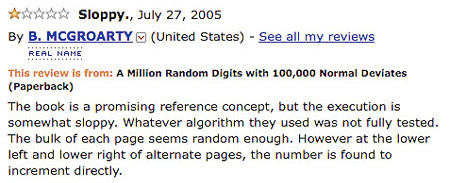
\includegraphics[height=3cm]{million_random_digits_review_1.jpg} \\

\includegraphics[height=3cm]{million_random_digits_review_2.jpg}
\end{figure}
\end{frame}

\begin{frame}{Motivation}
\textbf{True Random Number Generation} \\
Approaches:
\begin{itemize}
\pause \item Quantum effects
\pause \item Atmospheric noise
\pause \item ``Sonic Roulette Wheel'' (Rand)
\pause \item Human Input
\pause \item LavaRand
\end{itemize}
\vskip 0.5cm 
\begin{columns}
\column{0.35\textwidth}
\pause
Pro:
\begin{itemize}
\item aperiodic
\item nondeterministic
\item cryptographic security
\end{itemize}
\column{0.35\textwidth}
\pause
Con:
\begin{itemize}
\item blocking
\item not reproducible
\item costly to implement
\end{itemize}
\end{columns}
\end{frame}

\begin{frame}{Introduction}
\textbf{``Pseudorandom'' Number Generation}\\
\begin{displayquote}{Any one who considers arithemetical methods of producing random numbers is, of course, in a state of Sin. - John von Neumann}
\end{displayquote}
General Approach:
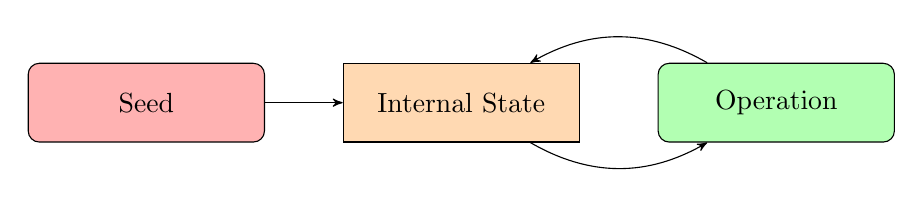
\begin{tikzpicture}[->,>=stealth', node distance=2cm]

\node (seed) [startstop] {Seed};
\node (internal_state) [process, right of=seed,  xshift=2cm] {Internal State};
\node (operation) [io, right of=internal_state, xshift=2cm] {Operation};

\path[every node/.style={font=\sffamily\small}]
    (seed) edge node [right] {} (internal_state)
    (internal_state) edge[bend right] node [left] {} (operation)
        (operation) edge[bend right] node [right] {} (internal_state);

\end{tikzpicture}
\pause
Key Attributes:
\begin{itemize}
\pause \item reproducible/deterministic
\pause \item quick to generate with common hardware
\pause \item independence (mostly)
\pause \item uniform distribution
\pause \item periodic
\end{itemize}
\end{frame}

\section{PRNG}

\subsection{Approaches to Uniform Random Number Generation}

\begin{frame}{Linear Congruence Method}
\textbf{Algorithm}
\begin{itemize}
\item choose ``magic numbers''
\begin{itemize}
\item \textbf{m}: modulo; $m > 0, m \subset \mathbb{Z}$ 
\item \textbf{a}: multiplier; $a > 0, a \subset \mathbb{Z}$
\item \textbf{c}: increment; $c \geq 0, a \subset \mathbb{Z}$
\end{itemize}
\item choose a ``seed:'' $\mathbb{X}_0$;  $0 \leq \mathbb{X}_0 < m, \mathbb{X}_0  \subset \mathbb{Z}$
\item generate $\mathbb{X}_n$ using the recursion relationship $\mathbb{X}_n = (\mathbb{X}_{n-1} \cdot a + c) \mod m$ (repeat as desired).
\end{itemize}
\end{frame}
\begin{frame}
\textbf{Example}
Let $m = 9$, $a = 4$, $c = 2$ $\mathbb{X}_0 = 2$.
\begin{table}
\centering
\begin{tabular}{l|c|c}
$n$ & $\mathbb{X}_n$ & $(\mathbb{X}_n \cdot a + c) \mod m$  \\\hline
0 & 4 & \pause $(4 \cdot 4 + 2) \mod 9 = 0$ \\
1 & 0 & \pause $(0 \cdot 4 + 2) \mod 9 = 2$ \\
2 & 2 & \pause $(2 \cdot 4 + 2) \mod 9 = 1$ \\
3 & 1 & $(1 \cdot 4 + 2) \mod 9 = 6$ \\
4 & 6 & $(6 \cdot 4 + 2) \mod 9 = 8$ \\
5 & 8 & $(8 \cdot 4 + 2) \mod 9 = 7$ \\
6 & 7 & $(7 \cdot 4 + 2) \mod 9 = 3$ \\
7 & 3 & $(3 \cdot 4 + 2) \mod 9 = 5$ \\
8 & 5 & $(5 \cdot 4 + 2) \mod 9 = 4$ \\
9 & 4 & \\
\end{tabular}
\end{table}

\end{frame}
\begin{frame}{Linear Congruence Method}
\textbf{Uniform Distribution:} 
\begin{itemize}
    \item let $p > 0 \subset \mathbb{Z}$ represent the period of a sequence $\mathbb{X}_0, ..., \mathbb{X}_{p - 1}$ generated using the linear congruence method
    \pause \item note that $\mathbb{X}_0 = \mathbb{X}_{p}$ [periodicity]
    \item note that $\forall n > 0 \subset \mathbb{Z}$, $\mathbb{X}_{n} < m$ [$\mathbb{X}_{n}$ generated by taking mod $m$]
    \item thus, $p \leq m$
   \pause \item under certain conditions on the ``magic numbers'' chosen, we are guaranteed that $p = m$ [i.e. the generator will take on its full period for all seed values]
    \pause \item let $0 < i, j < m = p, i \neq j$; $0 \leq \mathbb{X}_{i}, \mathbb{X}_{j} < m$ and $\mathbb{X}_{i} \neq \mathbb{X}_{j}$ implies $\forall q \subset \mathbb{Z} \text{ there exists a unique } n \text{ such that } \mathbb{X}_n = q$
\pause \item thus, as $m \rightarrow \infty$,  $E(\mathbb{X}/m) \rightarrow 1/2$
\pause \item similarly, it can be shown that $var(\mathbb{X}/m) \rightarrow 1/12$ (as expected for uniform distribution)

\end{itemize} 

\end{frame}

\begin{frame}{Linear Congruence Method}
\textbf{Independence:} 
\begin{itemize}
	\item lie on ``hyperplanes''
    \item severity depends on choice of ``magic numbers''
   	\begin{columns}
    \column{0.35\textwidth}
    \pause \item ``bad'' \\
    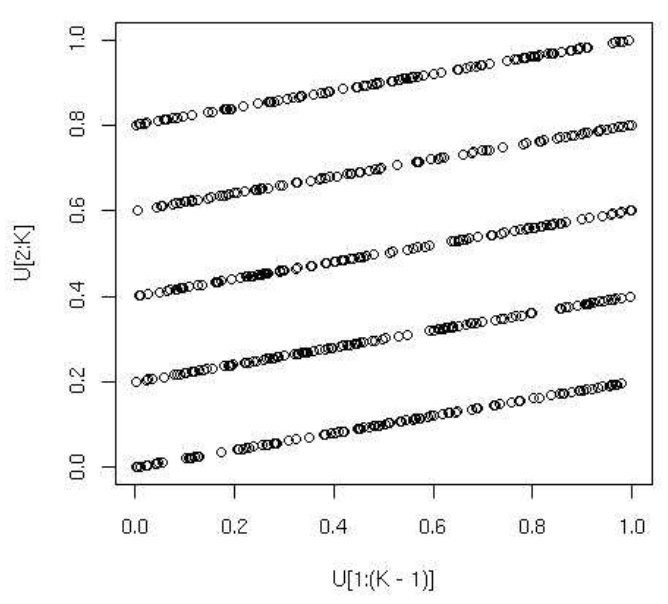
\includegraphics[height=3cm]{bad_distribution.jpg}
    \column{0.35\textwidth}
    \pause \item ``good'' \\
     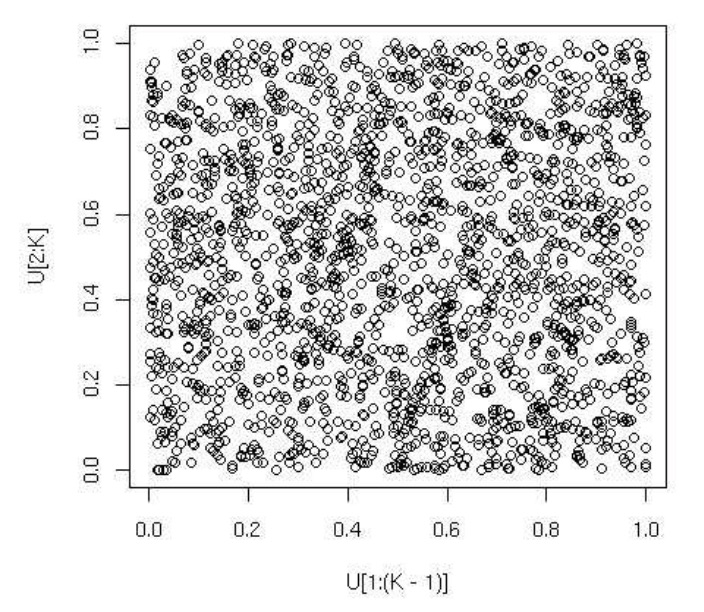
\includegraphics[height=3cm]{good_distribution.jpg}
     \end{columns}
    \pause \item thus, this generator may not be suitable for sensitive applications such as Monte Carlo methods
\end{itemize}
(image source: \url{http://www.mimuw.edu.pl/~apalczew/CFP_lecture3.pdf})
\end{frame}

\begin{frame}{Other Methods}
\pause \textbf{Mersenne Twister}
\begin{itemize}
\item 623-dimensional state vector
\item extremely long period: $2^{19937} − 1$
\item more guarantees about ``independence''
\item ``by far the most widely used general-purpose PRNG''
\end{itemize}

\pause \textbf{Blum Blum Shub}
\begin{itemize}
\item future outputs cannot be predicted from past outputs (cryptographic security)

\end{itemize}
\end{frame}

\subsection{Approaches to Non-Uniform Distributions}

\begin{frame}{Transformation Method}
Let $f(x)$ represent a pdf that we want to sample from.
Let $F(x)$ represent the cdf associated with that pdf.
Let $F^{-1}(y)$ represent the quantile function associated with that cdf.

Recall that $F^{-1}(y) (0,1) \rightarrow \mathbb{R}$.

\textbf{Algorithm:}
\begin{itemize}
\item Sample y = U[0,1].
\item Return $F^{-1}(y)$.
\end{itemize}

\end{frame}

\begin{frame}{Rejection Method}
For a pdf $f$ that we can't treat through the transformation method, choose a function $g$ such that:
\begin{itemize}
\item $\int_{-\infty}^{\infty}g(x)dx = A$ is finite
\item $g(x) \geq f(x)$ for all $x \subset \mathbb{R}$
\item we can select from $\frac{1}{A} g(x)$ using the transformation method or some other method
\end{itemize}
\pause \textbf{Algorithm:}
\begin{itemize}
\item select an $x$ from $\frac{1}{A}g(x)$
\item select a $y$ from $U[0,g(x)]$
\item if $y > f(x)$ reject and repeat from the top
\item else return $x$
\end{itemize}
The more tightly $g$ bounds $f$, the greater the efficiency of this approach (i.e. fewer rejected points).

\end{frame}

\section{Fin}
\begin{frame}{Conclusion}
\begin{centering}
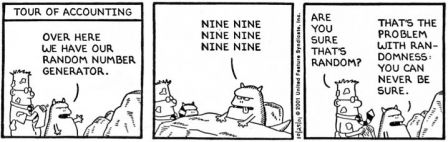
\includegraphics[height=3cm]{dilbert_cartoon.jpg} \\
\end{centering}
\end{frame}

\end{document}
